%%%%%%%%%%%%%%%%%%%%%%%%%%%%%%%%%%%%%%%
%%%%		Lab book
%%%%		Dylan Lawless 2020
%%%%%%%%%%%%%%%%%%%%%%%%%%%%%%%%%%%%%%%

%%%%%%%%%%%%%%%%%%
%		Labbook Settings
%		Dylan Lawless
%		2020
%%%%%%%%%%%%%%%%%%

\documentclass[a4paper,
								12pt,
								fleqn]{book}

\usepackage{listings} % for writing code verbatim. use \begin{lstlisting}
\usepackage{ccaption} % http://ctan.org/pkg/ccaption. This allows the legend placement on next page. May have problem with hyperref.
\usepackage[T1]{fontenc}
\usepackage[utf8]{inputenc}
\usepackage[english]{babel}
%\usepackage[french,german,english]{babel}

%%%%%%%%%%%%%%%%%%
%%%%	Index	%%%%
%%%%%%%%%%%%%%%%%%
\usepackage{imakeidx} % this one allows texmaker to make the index file. I believe the similar package \makeidx requires a separate step to run the index command. 
\makeindex %  this enables indexing commands. \printindex is used at the end of the main file after the bib. \printindex Can be in the contexts file instead too. 

% This is used to show the indext neatly on the page where it was sourced from. From someone on StackOverflow. It is used instead of the % \usepackage{showidx} which turns off the normal index printed at the end. 
\let\oldindex\index
\renewcommand{\index}[1]{\oldindex{#1}\marginpar{\small#1}}

%%%%%%%%%%%%%%%%%%
%%%%	Spacing	%%%%
%%%%%%%%%%%%%%%%%%
\usepackage{setspace} % increase interline spacing slightly
\setstretch{1.1} % my preferable size.

\makeatletter
\setlength{\@fptop}{0pt}  % for aligning all floating figures/tables etc... to the top margin
\makeatother

%%%%%%%%%%%%%%%%%%
%%%%	Table of contents	%%%%
%%%%%%%%%%%%%%%%%%
\setcounter{tocdepth}{4} %Sets the depth for TOC
\setcounter{secnumdepth}{0} % \setcounter{secnumdepth}{4} %Sets the numbering depth. -1 part, 0 chapter, 1 section, 2 subsection,  3 subsubsection, 4 paragraph, 5 subparagraph.

%The following three lines are included to add "Chapter" in front of the chapter number in the table of contents. Otherwise it would just read "1... 2.. etc"
\usepackage{tocloft,calc}
%\renewcommand{\cftchappresnum}{Chapter }
%\AtBeginDocument{\addtolength\cftchapnumwidth{\widthof{\bfseries Chapter }}}

%%%%%%%%%%%%%%%%%%
%%%% Formatting	%%%%
%%%%%%%%%%%%%%%%%%
\usepackage{amsmath} % For typesetting math
\usepackage{siunitx} %scientific units for measurements
\DeclareSIUnit\Molar{\textsc{m}} %scientific units for measurements molarity

%%%%%%%%%%%%%%%%%%
%%%%	Biblio	%%%%
%%%%%%%%%%%%%%%%%%
\usepackage[numbers,sectionbib,sort&compress]{natbib}  % sectionbib if to add bib per-chapter in conjuction with \usepackage{chapterbib}. Numbers is changing from the default author year to numbers. (Items in bibliography sorted in order cited). 
% natbib used in combination with style plainnat in the biblio file.

\setlength{\bibsep}{0.5pt}
\usepackage{chapterbib} % to add per-chapter bibliography.
\usepackage{notoccite}  % This is allowing citations to list in number of appearance 

%\usepackage[nottoc,numbib]{tocbibind}
	%Au­to­mat­i­cally adds the bib­li­og­ra­phy and/or the in­dex and/or the con­tents, etc., to the Ta­ble of Con­tents list­ing.
	
%%%%%%%%%%%%%%%%%%
%%%% Tables	%%%%
%%%%%%%%%%%%%%%%%%
\usepackage{tabularx}  % The same arguments as tabular*, but modifies the widths of certain columns, rather than the inter column space, to set a table with the requested total width. The columns that may stretch are marked with the new token X in the preamble argument.
\newcolumntype{Z}{ >{\centering\arraybackslash}X } % This preamble is used for centering in tabularx and X columns, i.e. the cntered heading box on a multi-column table. 

\usepackage{multirow} % This package is used in tables to make a column that spans vertically over several rows. Example use: for a coulm, 4 rows tall, with the work Test; {\multirow{4}{*}{Test}}.

\usepackage{ltablex} % this is to split table over multiple pages.

%%%%%%%%%%%%%%%%%%
%%%%	Drawings	%%%%
%%%%%%%%%%%%%%%%%%
\usepackage{qtree} 
	% this is for decision trees, or branching illustrastion etc. An example would be: $ \Tree [.S [ I [.VP use [.NP {\LaTeX} ]]]] 

\usepackage{tikz} %overlay caption and image or scale bar. 

\usepackage{textcomp}
	% to draw arrows in text mode use either command 
		% A$\,\to\,$B
		% A\textrightarrow B
		
\usepackage{wrapfig}

\usepackage{xymtexpdf} % chemical structures: for a simple ring structure use \cyclohexanev{}. This package's use of ; clashes with French for some reason. Apparently using a hack will work around: \begingroup \shorthandoff{;}  "formula here " \endgroup
		
%%%%%%%%%%%%%%%%%%
%%%%	Other formatting and color use	%%%%
%%%%%%%%%%%%%%%%%%
\usepackage{graphicx,xcolor}  % Required for including images
\graphicspath{{images/}}
\usepackage{courier} % to print font use \texttt{} 
\usepackage{subfig}
\usepackage{booktabs}
\usepackage{lipsum}
\usepackage{microtype}
\usepackage{url}
\usepackage[final]{pdfpages}

\usepackage{listings}
\lstset{language=[LaTeX]Tex,tabsize=4, basicstyle=\scriptsize\ttfamily, showstringspaces=false, numbers=left, numberstyle=\tiny, numbersep=10pt, breaklines=true, breakautoindent=true, breakindent=10pt}

\usepackage{hyperref}
\newcounter{dummy} % before a label \refstepcounter{dummy} is used to reset the counter and stop ref from linking to top of chapter.
\hypersetup{pdfborder={0 0 0},
	colorlinks=true,
	linkcolor={blue!50!black},
	citecolor={blue!50!black},
	urlcolor=black}
\urlstyle{same}

\makeatletter
\def\cleardoublepage{\clearpage\if@twoside \ifodd\c@page\else
    \hbox{}
    \thispagestyle{empty}
    \newpage
    \if@twocolumn\hbox{}\newpage\fi\fi\fi}
\makeatother \clearpage{\pagestyle{plain}\cleardoublepage}

%%%%%%%%%%%%%%%%%%
%%%%% Chapter Header %%%%
%%%%%%%%%%%%%%%%%%
\usepackage{color}
\usepackage{tikz}
\usepackage[compact]{titlesec} %\usepackage[explicit]{titlesec}
 
%\newcommand*\chapterlabel{}
%%\renewcommand{\thechapter}{\Roman{chapter}}
%\titleformat{\chapter}[display]  % type (section,chapter,etc...) to vary,  shape (eg display-type)
%	{\normalfont\bfseries\Huge} % format of the chapter
%	{\gdef\chapterlabel{\thechapter\ }}     % the label 
% 	{0pt} % separation between label and chapter-title
% 	  {\begin{tikzpicture}[remember picture,overlay]
%    \node[yshift=-8cm] at (current page.north west)
%      {\begin{tikzpicture}[remember picture, overlay]
%        \draw[fill=black] (0,0) rectangle(35.5mm,15mm);
%        \node[anchor=north east,yshift=-7.2cm,xshift=34mm,minimum height=30mm,inner sep=0mm] at (current %page.north west)
%        {\parbox[top][30mm][t]{15mm}{\raggedleft $\phantom{\textrm{l}}$\color{white}\chapterlabel}};  %the black l is just %to get better base-line alingement
%        \node[anchor=north west,yshift=-7.2cm,xshift=37mm,text width=\textwidth,minimum height=30mm,inner %sep=0mm] at (current page.north west)
%              {\parbox[top][30mm][t]{\textwidth}{\color{black}#1}};
%       \end{tikzpicture}
%      };
%   \end{tikzpicture}
%   \gdef\chapterlabel{}
%  } % code before the title body

% \titleformat{\chapter}[display]
%   {\normalfont\bfseries}{\chaptertitlename\ \thechapter}{20pt}{}
  
\titleformat{\section}[display]
  {\normalfont\bfseries}{\sectiontitlename\ \thesection}{20pt}{}

\titleformat{\subsection}[display]
  {\normalfont\bfseries}{\sectiontitlename\ \thesection}{20pt}{}
    
\titlespacing*{\chapter}{0pt}{0pt}{0pt} % I want to remove excess spacing 
%\titlespacing*{\section}{0pt}{13.2pt}{*0}  % 13.2pt is line spacing for a text with 11pt font size
%\titlespacing*{\subsection}{0pt}{13.2pt}{*0}
%\titlespacing*{\subsubsection}{0pt}{13.2pt}{*0}

%\newcounter{myparts}
%\newcommand*\partlabel{}
%\titleformat{\part}[display]  % type (section,chapter,etc...) to vary,  shape (eg display-type)
%	{\normalfont\bfseries\Huge} % format of the part
%	{\gdef\partlabel{\thepart\ }}     % the label 
% 	{0pt} % separation between label and part-title
% 	  {\setlength{\unitlength}{20mm}
%	  \addtocounter{myparts}{1}
%	  \begin{tikzpicture}[remember picture,overlay]
%    \node[anchor=north west,xshift=-65mm,yshift=-6.9cm-\value{myparts}*20mm] at (current page.north east) % for %unknown reasons: 3mm missing -> 65 instead of 62
%      {\begin{tikzpicture}[remember picture, overlay]
%        \draw[fill=black] (0,0) rectangle(62mm,20mm);   % -\value{myparts}\unitlength
%        \node[anchor=north west,yshift=-6.1cm-\value{myparts}*20mm,xshift=-60.5mm,minimum height=30mm,inner %sep=0mm] at (current page.north east)
%        {\parbox[top][30mm][t]{55mm}{\raggedright \color{white}Part \partlabel $\phantom{\textrm{l}}$}};  %the phantom l %is just to get better base-line alingement
%        \node[anchor=north east,yshift=-6.1cm-\value{myparts}*20mm,xshift=-63.5mm,text width=\textwidth,minimum height=30mm,inner sep=0mm] at (current page.north east)
%              {\parbox[top][30mm][t]{\textwidth}{\raggedleft \color{black}#1}};
%       \end{tikzpicture}
%      };
%   \end{tikzpicture}
%   \gdef\partlabel{}
%  } % code before the title body

%%%%%%%%%%%%%%%%%%
%%%%% New settings for labbook %%%%
%%%%%%%%%%%%%%%%%%
\usepackage[bottom=10em, margin=4cm]{geometry} % Marging make the horizontal space smaller for quick reading. Bottom size reduces the whitespace at the bottom of the page so more text can fit

\usepackage{marginnote} % used after loading geometry. 

%\usepackage[osf]{mathpazo} % Palatino as the main font
%\linespread{1.05}\selectfont % Palatino needs some extra spacing, here 5% extra
%\usepackage[scaled=.88]{beramono} % Bera-Monospace
%\usepackage[scaled=.86]{berasans} % Bera Sans-Serif

%\usepackage{booktabs,array} % Packages for tables

\usepackage{etoolbox}
%\usepackage[norule]{footmisc} % Removes the horizontal rule from footnotes
\usepackage{lastpage} % Counts the number of pages of the document

% Print chapters on same page instead of starting on fresh pages. Use \usepackage{etoolbox} and remove the clear double page after chapters
%\makeatletter
%\patchcmd{\chapter}{\if@openright\cleardoublepage\else\clearpage\fi}{}{}{}
%\makeatother

% Paragraph indent setting
% \setlength{\parindent}{0pt}

% I want a page header with a hyperlink to jump to the most current entry. fancyhdr will allow this kind of header. 
\usepackage{fancyhdr} 
\fancyhf{}
\cfoot{\thepage}
\pagestyle{fancy} 

%%%%%%%%%%%%%%%%%%
%%%%	Make a command for labelling the daily project title	%%%%
%%%%%%%%%%%%%%%%%%
% My projects are called "A" and "B"

\newcommand{\projectA}[1]{{\color{purple} \bf{projectA}}}
\newcommand{\projectB}[1]{{\color{teal}{projectB}}}

\newcommand{\labday}{\section}% \labday will be replaced with \section. However, the "labday" does not show up as a heading in the texmaker Structure panel. 





%%%% Other	%%%%
%\usepackage[dvipsnames]{xcolor}  % Allows the definition of hex colors
%\definecolor{titleblue}{rgb}{0.16,0.24,0.64} % Custom color for the title on the title page
%\definecolor{linkcolor}{rgb}{0,0,0.42} % Custom color for links - dark blue at the moment

%\usepackage{scrlayer-scrpage} % part of the KOMA-script bundle. Using this package to customize the headers and footers is recommended with every KOMA-script class. The package can be used with the standard classes as well.

%\addtokomafont{title}{\Huge\color{titleblue}} % Titles in custom blue color
%\addtokomafont{chapter}{\color{OliveGreen}} % Lab dates in olive green
%\addtokomafont{section}{\color{Sepia}} % Sections in sepia
%\addtokomafont{pagehead}{\normalfont\sffamily\color{gray}} % Header text in gray and sans serif
%\addtokomafont{caption}{\footnotesize\itshape} % Small italic font size for captions
%\addtokomafont{captionlabel}{\upshape\bfseries} % Bold for caption labels
%\addtokomafont{descriptionlabel}{\rmfamily}
%\setcapwidth[r]{10cm} % Right align caption text
%\setkomafont{footnote}{\sffamily} % Footnotes in sans serif

% \deffootnote[4cm]{4cm}{1em}{\textsuperscript{\thefootnotemark}} % Indent footnotes to line up with text

% \DeclareFixedFont{\textcap}{T1}{phv}{bx}{n}{1.5cm} % Font for main title: Helvetica 1.5 cm
% \DeclareFixedFont{\textaut}{T1}{phv}{bx}{n}{0.8cm} % Font for author name: Helvetica 0.8 cm

%\usepackage[nouppercase,headsepline]{scrpage2} % Provides headers and footers configuration
%\pagestyle{scrheadings} % Print the headers and footers on all pages
%\clearscrheadfoot % Clean old definitions if they exist

%\automark[chapter]{chapter}
%\ohead{\headmark} % Prints outer header

%\setlength{\headheight}{25pt} % Makes the header take up a bit of extra space for aesthetics
%\setheadsepline{.4pt} % Creates a thin rule under the header
%\addtokomafont{headsepline}{\color{lightgray}} % Colors the rule under the header light gray

%\ofoot[\normalfont\normalcolor{\thepage\ |\  \pageref{LastPage}}]{\normalfont\normalcolor{\thepage\ |\  %\pageref{LastPage}}} % Creates an outer footer of: "current page | total pages"

% These lines make it so each new lab day directly follows the previous one i.e. does not start on a new page - comment them out to separate lab days on new pages
%\makeatletter
%\patchcmd{\addchap}{\if@openright\cleardoublepage\else\clearpage\fi}{\par}{}{}
%\makeatother
%\renewcommand*{\chapterpagestyle}{scrheadings}

% These lines make it so every figure and equation in the document is numbered consecutively rather than restarting at 1 for each lab day - comment them out to remove this behavior
%\usepackage{chngcntr}
%\counterwithout{figure}{labday}
%\counterwithout{equation}{labday}


%%%%%%%%%%%%%%%%%%%%%%%%%%%%%%%%%%%%%%%%%%%%%%%
%% EDOC THESIS TEMPLATE: Variant 1.0 -> Latin modern, large text width&height
%%%%%%%%%%%%%%%%%%%%%%%%%%%%%%%%%%%%%%%%%%%%%%%
%\usepackage{lmodern}
%\usepackage[a4paper,top=22mm,bottom=28mm,inner=35mm,outer=25mm]{geometry}
%%%%%%%%%%%%%%%%%%%%%%%%%%%%%%%%%%%%%%%%%%%%%%%

%%%%%%%%%%%%%%%%%%%%%%%%%%%%%%%%%%%%%%%%%%%%%%
% EDOC THESIS TEMPLATE: Variant 2.0 -> Utopia, Gabarrit A (lighter pages)
%%%%%%%%%%%%%%%%%%%%%%%%%%%%%%%%%%%%%%%%%%%%%%
%\usepackage{fourier} % Utopia font-typesetting including mathematical formula compatible with newer TeX-Distributions (>2010)
%\usepackage{utopia} % on older systems -> use this package instead of fourier in combination with mathdesign for better looking results
%\usepackage[adobe-utopia]{mathdesign}

%\setlength{\textwidth}{146.8mm} % = 210mm - 37mm - 26.2mm
%\setlength{\oddsidemargin}{11.6mm} % 37mm - 1in (from hoffset)
%\setlength{\evensidemargin}{0.8mm} % = 26.2mm - 1in (from hoffset)
%\setlength{\topmargin}{-2.2mm} % = 0mm -1in + 23.2mm 
%\setlength{\textheight}{221.9mm} % = 297mm -29.5mm -31.6mm - 14mm (12 to accomodate footline with pagenumber)
%\setlength{\headheight}{14pt}
%%%%%%%%%%%%%%%%%%%%%%%%%%%%%%%%%%%%%%%%%%%%%%


% custom packages, etc. in this file

%%%%%%%%%%%%%%%%%%%%%%%%%%%%%%%%%%%%%%%
%%%% HEAD: Book-Begin                  %%%%
%%%%%%%%%%%%%%%%%%%%%%%%%%%%%%%%%%%%%%%

\begin{document}
\frontmatter
\begin{titlepage}
\begin{center}
%\large
%\sffamily

\null\vspace{2cm}
\Large Laboratory book \\[24pt]
{\textcolor{gray}{\normalsize{Dylan Lawless}}}
    
\vfill
	École polytechnique fédérale de Lausanne\\
	
\includegraphics[width=2cm]{images/EPFL_Logo_Digital_RGB_PROD}		
\vfill
	
	Start Aug 2020\\

\end{center}
\vspace{2cm}
\end{titlepage}
\chapter*{Publication Statement}
\markboth{Publication Statement}{Publication Statement}
\addcontentsline{toc}{chapter}{Publication Statement}
This lab book concerns two projects are explicitly labelled by color as {\color{purple} \bf{projectA}} and {\color{teal} \bf{projectB}}  as well as several other non-specified projects, and day-to-day notes and ideas. 

The author confirms that the work submitted is their own, except where work which has formed part of jointly-authored publications has been included. 
The author confirms that appropriate credit has been given within this document where reference has been made to the work of others.

This copy has been produced on the understanding that it is copyright material and that no quotation from the thesis may be published without proper acknowledgements.

% The right of the Author as named on the cover page has been asserted by them in accordance with the Copyright, Designs and Patents Act 1988.
\clearpage
%\input{head/acknowledgements}
%\include{head/abstracts}
\clearpage
\tableofcontents
\clearpage

%%%%	Table and figure TOC %%%%
% \listoffigures
% \addcontentsline{toc}{chapter}{List of figures} % adds an entry to the table of contents
% \listoftables
% \addcontentsline{toc}{chapter}{List of tables} % adds an entry to the table of contents

% \setlength{\parskip}{1em} % space before each new paragraph (needs to be after titlepage and frontmatter to keep the table of contents lists short)

%%%%%%%%%%%%%%%%%%%%%%%%%%%%%%%%%%%%%%%
%%%%	MAIN: The contents of the labbook  %%%%
%%%%%%%%%%%%%%%%%%%%%%%%%%%%%%%%%%%%%%%
\mainmatter
\newpage
% \include{main/ch_abbreviations}
\pagestyle{myheadings}
\markboth{\nameref{sec:End}}{\nameref{sec:End}}

\chapter{Lab book 2020}

\section{Introduction}
%\markboth{Introduction}{Introduction}
%\addcontentsline{toc}{chapter}{Introduction}
Stuff about eigenvectors\index{eigenvector} and
eigenvalues\index{eigenvalue} which are being  indexed at the end of this book. 

The current classification of primary immunodeficiencies (PIDs) was compiled by the Expert Committee of the International Union of Immunological Societies
\citep{picard2018international}
in \textit{The Primary Immunodeficiency Diseases Committee Report on Inborn Errors of Immunity}.
Over approximately 50 years the list of inborn errors of immunity has grown to over 350 disorders.
I use vim snippets in my .vimrc: for producing formatting quickly including, bold face, italics, headings, and code.

\begin{lstlisting}
Computer code like this is writtin using the command. begin{lstlisting} and end{lstlisting}.
\end{lstlisting}
\marginnote{This is a margin note using the geometry package, set at 
3cm vertical offset to the line it is typeseted.}%[3cm]
Footnote example\footnote{Lorem ipsum dolor sit amet, consectetuer adipiscing elit.}.\\

\section{Sat, 8 Aug 2020 \projectA{} } 
I will add margin note after some placeholder text.
\lipsum[2-3]

\marginnote{The R script used is in "viral sequence / phylo / tree.r"}

\section{Mon, 10 Aug 2020 \projectB{}}
Working on the phylogenetic trees. 
I am producing phylogenetic trees and then splitting based on the obvious clade groups, add color, and add all labels. 
I used ggtree and ape for this work.\\
\url{ https://yulab-smu.github.io/treedata-book} \\
\url{https://4va.github.io/biodatasci/r-ggtree.html}\\
Index: phylogenetic tree, ggtree, ape.
\index{phylogenetic tree}
\index{ggtree}
\index{ape}

\section{Fri 14 Aug \projectB{} }
Here are some specific notes on a recent task.

\subsection{Processing viral data}
For \projectB{} I used ncbi-tools-bin to convert to fasta format
(note the software "Sequin" does the same job but it GUI only).
\url{https://www.huge-man-linux.net/man1/asn2fsa.html}
\index{ncbi-tools}
\begin{lstlisting}
sudo apt-get install ncbi-tools-bin
for file in rsv.*.sqn; do asn2fsa -a a -i $file -v $file.fa; done
dir: ./fa
\end{lstlisting}

Each viral genome has 11 segments that are sequenced.
With awk, I split each fasta to a new file and labelled with the read name.
i.e. segment 1 for all samples is in the file seg\_1, etc.
used \$split.sh
dir: ./seg
redo this step and split based on whole line name per fasta (remove spaces)
I used the macOS command line version of muscle to align, printing out clustal format
\begin{lstlisting}
$ for file in seg_*; do ~/Desktop/muscle3.8.31_i86darwin64 -in $file -clw -out clw.$file; done
dir: ./clw
\end{lstlisting}

I had ncbi-tools-bin installed since it runs on Debian.
I will try on my local macOS.
\url{https://ftp.ncbi.nlm.nih.gov/toolbox/ncbi_tools/}
\begin{lstlisting}
mv mac.asn2fsa ./tools/
mkdir rsv_viral_sequence_local
sync sqn dir from scitas

To extract the nucleotide from sqn.
1.export_nucleotide.sh
#!/bin/bash
# output options -v for amino, -o for nucleotide.
cd sqn
for file in rsv.*.sqn;
    do ~/tools/mac.asn2fsa -a a -i $file -o ${file%.*}.nt.fa;
done
mv ./*.nt.fa ../nt
\end{lstlisting}

Then make a simple header.
\begin{lstlisting}
$ cat 2.simplify_header.sh
#!/bin/bash
cd ./nt
for file in *.nt.fa;
    do awk -F" " '/>/{$0=$1}1' $file > ${file%.*}.nt_smp.fa ;
    done

mv ./*.nt_smp.fa ../nt_simple/

move all to post/inspire/viral_sequence/rsv_viral_seq/
\end{lstlisting}

\section{Fri, 27 Aug Lab meeting}
\subsection{Second gen P-value}
\begin{figure}[!h]
\begin{center}
  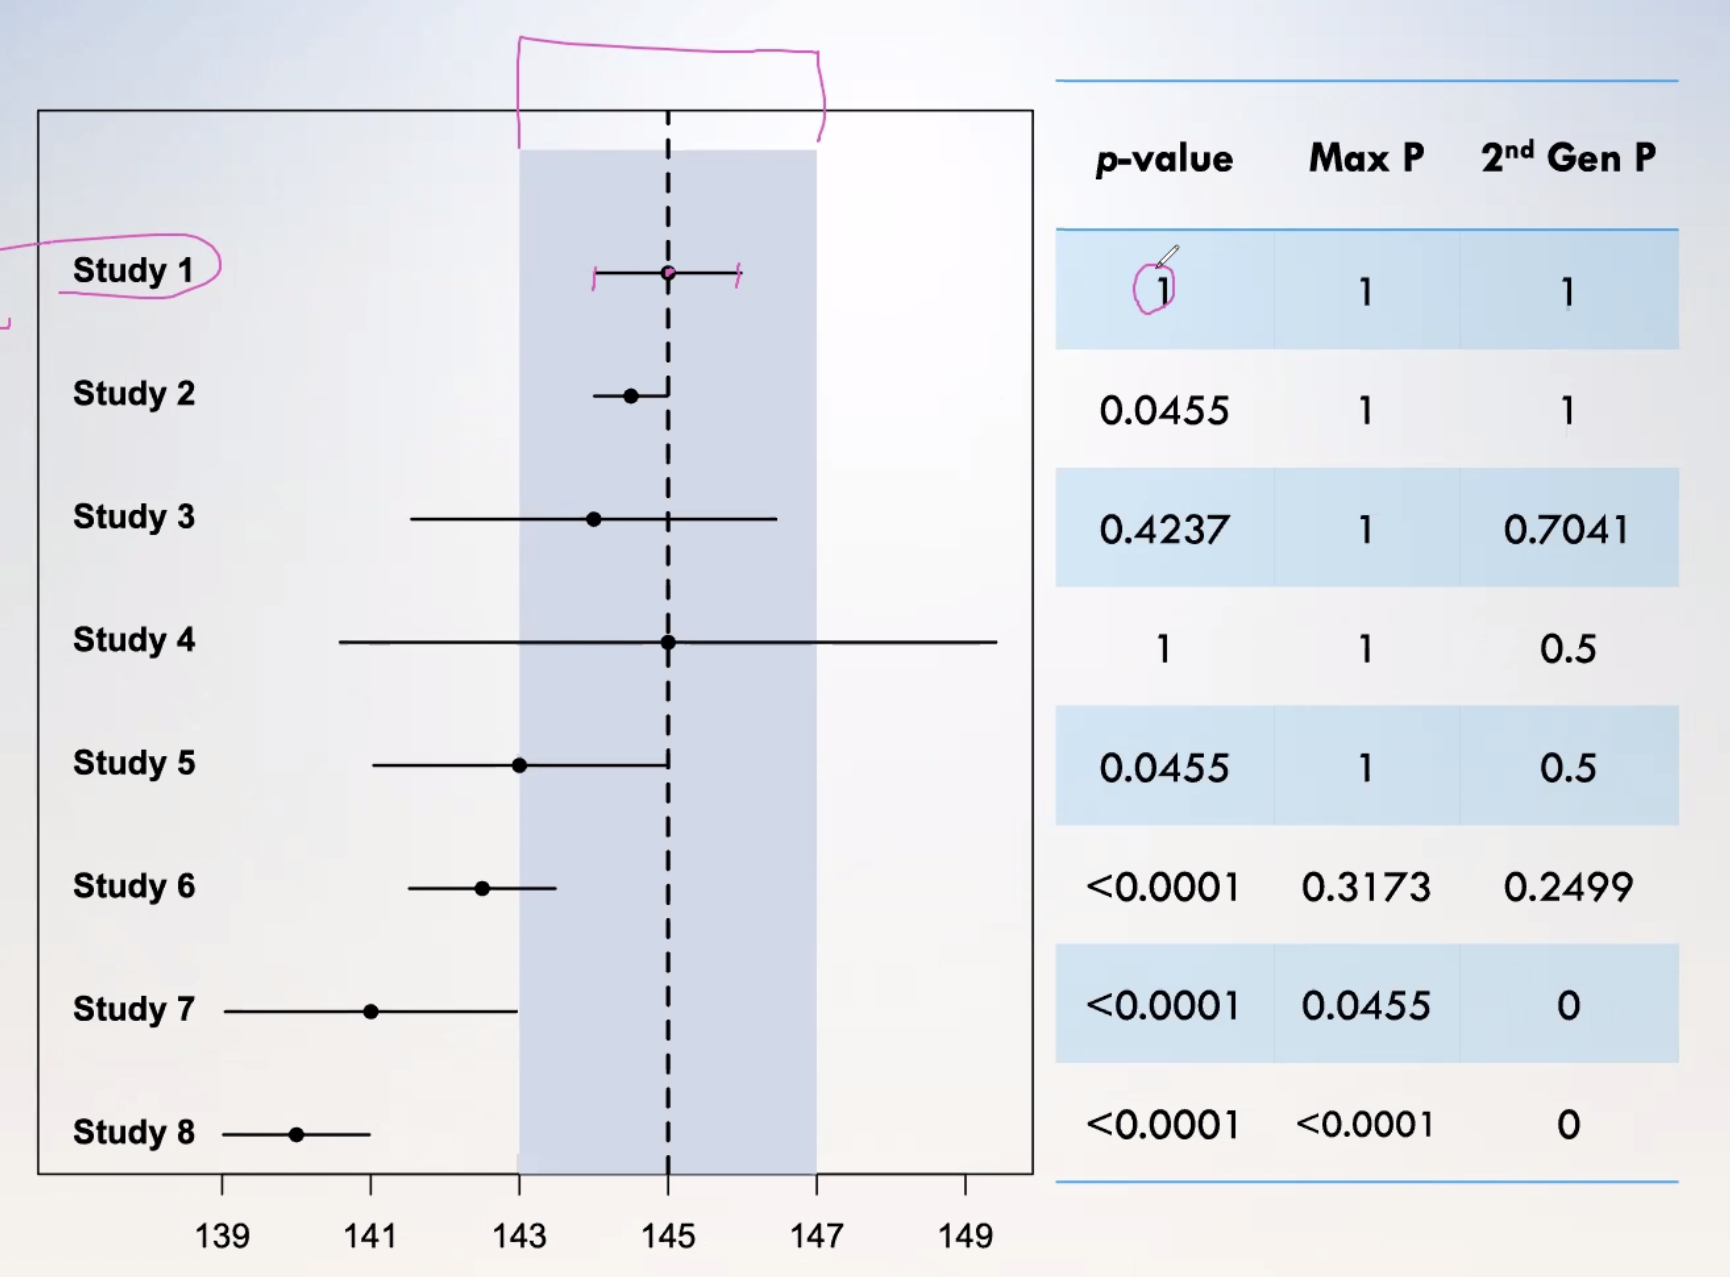
\includegraphics[scale=0.1]{misc/sgpv}
    \caption[Second gen P val]{\textbf{Second gen P val.} }
  \end{center}
\end{figure}

% Add place holder text to fill up pages and view the layout.
\lipsum[2-10]


\pagestyle{myheadings}
\markboth{\nameref{sec:End}}{\nameref{sec:End}}

\chapter{Methods and tools}
\section{Imputation}
%\markboth{Introduction}{Introduction}
%\addcontentsline{toc}{chapter}{Introduction}
Genipe Imputation pipeline tutorial
\url{http://pgxcentre.github.io/genipe/index.html}
\index{Imputation}

\section{Burden test / SKAT}
SKAT 
\citet{Lee2012Optimal}
and SKAT-O 
\citet{Lee2012Optimalunified} (I believe this is correct but check).
Author homepage
\url{https://www.hsph.harvard.edu/skat/}
Some info on the methods from Golden helix 
\url{https://doc.goldenhelix.com/SVS/tutorials/variant_analysis/skatAndSkato.html}.
Package in R 
\url{https://cran.r-project.org/web/packages/SKAT/SKAT.pdf}
\index{SKAT}
A different paper on burden testing
\url{https://www.ncbi.nlm.nih.gov/pmc/articles/PMC6174288/}.

\section{}




\section{Go to End} \refstepcounter{dummy} \label{sec:End} % Marker for page header shortcut to most recent entry.

%%%%%%%%%%%%%%%%%%%%%%%%%%%%%%%%%%%%%%%
%%%%% TAIL: Bibliography, Appendix, CV  %%%%%
%%%%%%%%%%%%%%%%%%%%%%%%%%%%%%%%%%%%%%%

\bibliographystyle{unsrtnat}
\bibliography{tail/labbook_bibliography}
\addcontentsline{toc}{section}{Bibliography}

\printindex
\addcontentsline{toc}{section}{Index}

%\appendix
\chapter{An appendix}

\lipsum[1]

% \include{tail/labbook_bibliography}
%\include{tail/biblio}
		%% While using chapterbib / sectionbib Run LATEX; run BibTEX on each included file; run LATEX; run LATEX. 
		%% For normal bib, silence the per-chapter bibliography and rely on normal use of the bib in this main root file. 
% Add your glossary here
% Add your index here
%\include{tail/publications}

\end{document}
